%!TEX root = ./main.tex

\section{Intro}
\addtocounter{minutes}{2}
\begin{frame}%
	\frametitle{Intro}%
	%\framesubtitle{}
    Initiatief van studenten
	\vspace{0.2cm}
	
   	\centering%
   	\begin{minipage}{0.30\linewidth}%
        \centering%
		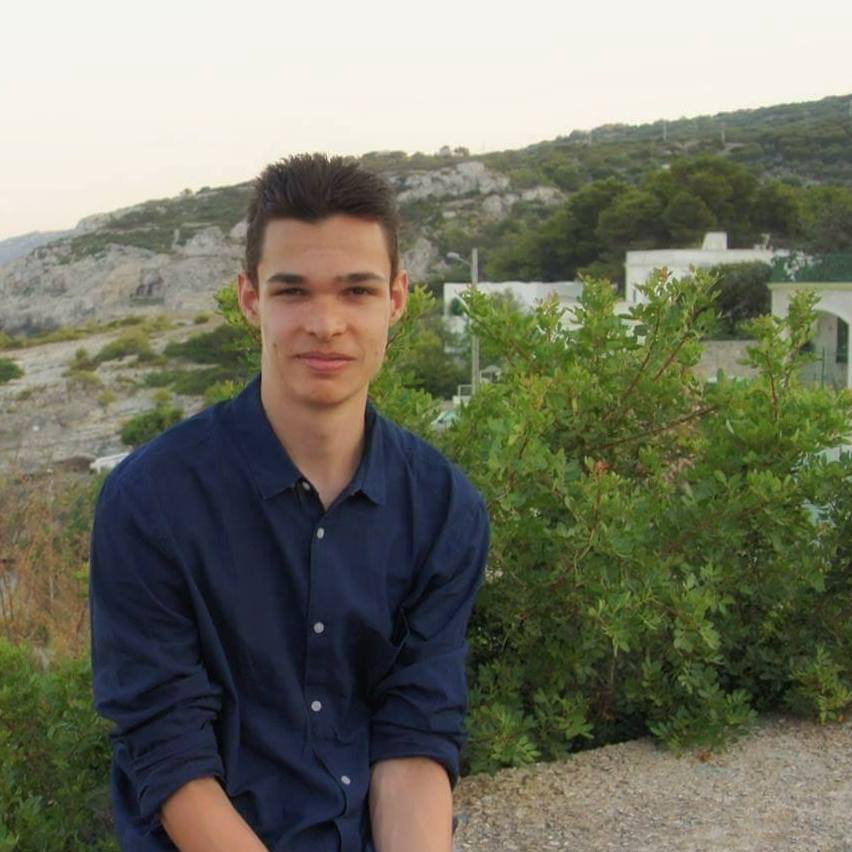
\includegraphics[width=\linewidth]{res/stijn} \\%
        \footnotesize Stijn Rosaer -1Ma\strut%
    \end{minipage}
    \begin{minipage}{0.30\linewidth}%
        \centering%
		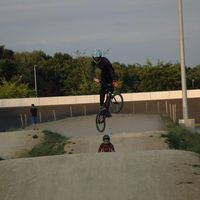
\includegraphics[width=\linewidth]{res/sam} \\%
        \footnotesize Sam Pieters -2Ba \strut%
    \end{minipage}
    \begin{minipage}{0.30\linewidth}%
        \centering%
		
\includegraphics[width=\linewidth]{res/mateo} \\%
        \footnotesize Mateo Sierens -3Ba\strut%
    \end{minipage}
    \begin{minipage}{0.30\linewidth}%
        \centering%
        \noindent
\includegraphics[width=\linewidth]{res/arno} \\%
        \footnotesize Arno Deceuninck -3Ba\strut%
    \end{minipage}  	
    \begin{minipage}{0.30\linewidth}%
        \centering%
		
\includegraphics[width=\linewidth]{res/senne} \\%
        \footnotesize Senne Rosaer -1Ma\strut%
    \end{minipage}
    \begin{minipage}{0.30\linewidth}%
		\centering%
		
\includegraphics[width=\linewidth]{res/toon} \\%
		\footnotesize Toon Meynen -1Ma\strut%
    \end{minipage}
\end{frame}  

\section{Planning}
\addtocounter{minutes}{3}
\begin{frame}
	\frametitle{Planning}
    \includeSchedule
    
	% NOTE: Volgende sessie:  Dual boot $->$ USB stick en laptop

\end{frame}

\section{Blackboard}
\begin{frame}
    \frametitle{Blackboard}
    
\includegraphics[scale=0.5]{res/bb.png}    

	
	Blackboard cursus Hitchhikers guide to computer science
	\vspace{1cm}

	Contacteer ons indien niet zichtbaar!\\
	\texttt{stijn.rosaer@student.uantwerpen.be}
\end{frame}

\section{Facebook}
\begin{frame}
	\frametitle{Faceboek groep}
	\begin{center}
		
\includegraphics[scale=0.7]{res/qrfb.png}
	\end{center}
\end{frame}

\section{Eerste sessie}
\begin{frame}
	\frametitle{Eerste sessie}
	\textbf{Donderdag 24 september}\\
	\vspace{1cm}
	
	\begin{center}
	\begin{tabular}{c|c|c}
    Groep A & G.004 & 10:45\\
    Groep B & G.006 & 10:45\\ \hline
    Groep C & G.004 & Na CSA\\
    Groep D & G.006 & Na CSA
    \end{tabular}
	\end{center}
    
\end{frame}







